\section{Example: Skew-Rotation}

\begin{frame}
	Fix $a \in \mathbb{R} \setminus \mathbb{Q}$ and look at $\mathbb{T}^2 = \mathbb{R}/\mathbb{Z} \times \mathbb{R}/\mathbb{Z}$ with the skew rotation $\beta: \mathbb{T}^2 \to \mathbb{T}^2$ with
	\begin{align*}
		\beta([x_1], [x_2]) := ([x_1+a], [x_2+x_1]).
	\end{align*}

	The arising TDS $(\mathbb{T}^2, \mathbb{Z})$ is minimal and not equicontinuous.
	
	\begin{figure}[h]
		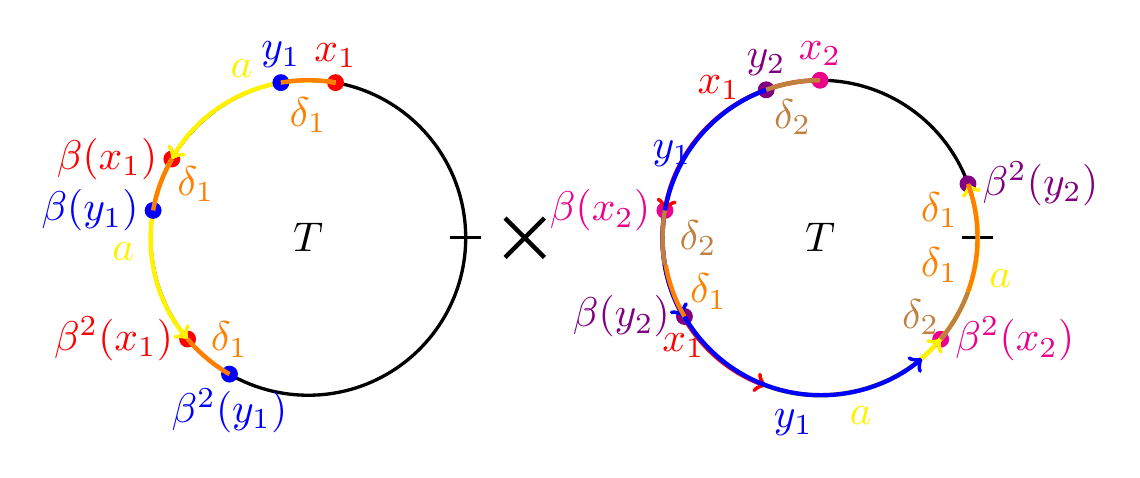
\begin{tikzpicture}
			\draw[very thick] (0, 0) circle (2) node[scale=1.5] {$\mathbb{T}$};
			\draw[very thick] (1.8, 0) -- (2.2, 0);
			
			\filldraw[color=red] (.347, 1.970) circle (.1) node[anchor=south, scale=1.5] {$x_1$};
			\filldraw[color=red] (-1.732, 1) circle (.1) node[anchor=east, scale=1.5] {$\beta(x_1)$};
			\filldraw[color=red] (-1.532, -1.286) circle (.1) node[anchor=east, scale=1.5] {$\beta^2(x_1)$};
			
			\draw[ultra thick, color=yellow, ->] (.347, 1.970) arc (80:150:2) node[above, midway, scale=1.5] {$a$};
			\draw[ultra thick, color=yellow, ->] (-1.732, 1) arc (150:220:2) node[left, midway, scale=1.5] {$a$};
			
			\filldraw[color=blue] (-.347, 1.970) circle (.1) node[anchor=south, scale=1.5] {$y_1$};
			\filldraw[color=blue] (-1.970, .347) circle (.1) node[anchor=east, scale=1.5] {$\beta(y_1)$};
			\filldraw[color=blue] (-1, -1.732) circle (.1) node[anchor=north, scale=1.5] {$\beta^2(y_1)$};
			
			\draw[ultra thick, color=orange] (.347, 1.970) arc (80:100:2) node[below, midway, scale=1.5] {$\delta_1$};
			\draw[ultra thick, color=orange] (-1.732, 1) arc(150:170:2) node[right, midway, scale=1.5] {$\delta_1$};
			\draw[ultra thick, color=orange] (-1.532, -1.286) arc(220:240:2) node[above, scale=1.5] {$\delta_1$};
			
			
			\draw[ultra thick] (2.5, .25) -- (3, -.25);
			\draw[ultra thick] (2.5, -.25) -- (3, .25);
			
			
			\draw[very thick] (6.5, 0) circle (2) node[scale=1.5] {$\mathbb{T}$};
			\draw[very thick] (8.3, 0) -- (8.7, 0);
			
			\filldraw[color=magenta] (6.5, 2) circle (.1) node[anchor=south, scale=1.5] {$x_2$};
			\filldraw[color=magenta] (4.530, .347) circle (.1) node[anchor=east, scale=1.5] {$\beta(x_2)$};
			\filldraw[color=magenta] (8.032, -1.289) circle (.1) node[anchor=west, scale=1.5] {$\beta^2(x_2)$};
			
			\draw[ultra thick, color=red, ->] (6.5, 2) arc (90:170:2) node[above, midway, scale=1.5] {$x_1$};
			\draw[ultra thick, color=red, ->] (4.530, .347) arc(170:250:2) node[below, midway, scale=1.5] {$x_1$};
			\draw[ultra thick, color=yellow, ->] (5.816, -1.879) arc(250:320:2) node[below, midway, scale=1.5] {$a$};
			
			\filldraw[color=violet] (5.816, 1.879) circle (.1) node[anchor=south, scale=1.5] {$y_2$};
			\filldraw[color=violet] (4.778, -1) circle (.1) node[anchor=east, scale=1.5] {$\beta(y_2)$};
			\filldraw[color=violet] (8.379, .684) circle (.1) node[anchor=west, scale=1.5] {$\beta^2(y_2)$};
			
			\draw[ultra thick, color=blue, ->] (5.816, 1.879) arc (110:210:2) node[above, midway, scale=1.5] {$y_1$};
			\draw[ultra thick, color=blue, ->] (4.778, -1) arc (210:310:2) node[below, midway, scale=1.5] {$y_1$};
			\draw[ultra thick, color=yellow, ->] (7.786, -1.532) arc(310:380:2) node[right, midway, scale=1.5] {$a$};
			
			\draw[ultra thick, color=brown] (6.5, 2) arc (90:110:2) node[below, midway, scale=1.5] {$\delta_2$};
			\draw[ultra thick, color=brown] (4.530, .347) arc (170:190:2) node[right, midway, scale=1.5] {$\delta_2$};
			\draw[ultra thick, color=orange] (4.778, -1) arc (210:190:2) node[right, midway, scale=1.5] {$\delta_1$};
			\draw[ultra thick, color=brown] (8.032, -1.289) arc (320:340:2) node[left, midway, scale=1.5] {$\delta_2$};
			\draw[ultra thick, color=orange] (8.5, 0) arc (360:340:2) node[left, midway, scale=1.5] {$\delta_1$};
			\draw[ultra thick, color=orange] (8.5, 0) arc(0:20:2) node[left, midway, scale=1.5] {$\delta_1$};
		\end{tikzpicture}
	\end{figure}
\end{frame}

\begin{frame}
	\begin{example}
		The MEF of the skew-ration $(\mathbb{T}^2, \beta)$ is given by the circle rotation $(\mathbb{T}, \alpha)$ with factor map $\pi$ given by $([x_1], [x_2]) \mapsto [x_1]$.
	\end{example}
	We need to prove that
	\begin{align*}
		Q_2(\mathbb{T}^2) = R_\pi = \{(([x_1], [x_2]), ([y_1], [y_2])) \in \mathbb{T}^2 \times \mathbb{T}^2;\ [x_1] = [y_1]\}.
	\end{align*}
	\medskip

	We already know that $(\mathbb{T}, \alpha)$ is equicontinuous, which implies $Q_2(\mathbb{T}^2) \subseteq R_\pi$.
\end{frame}

\begin{frame}
	For the other direction we prove that $(([z], [x]), ([z], [y])) \in R_\pi$ is regional proximal.
	\medskip
	
	Fix $\varepsilon > 0$. W.l.o.g. $0 \leq x \leq y < 1$. Choose some $0 < b < \frac{\varepsilon}{2}$ and $n \in \mathbb{N}$ such that
	\begin{align*}
		0 < (y-x) - nb < \frac{\varepsilon}{2}.
	\end{align*}
	\medskip
	
	Then $([z+b], [x])$ and $([z], [y])$ are in the $\varepsilon$ neighborhoods of $([z], [x])$ and $([z], [y])$ respectively and
	\begin{align*}
		&d_{\mathbb{T}^2}(\beta^n([z+b], [x]), \beta^n([z], [y]))\\
		= &d_{\mathbb{T}^2}(([z+b+na], [x + n(z+b) + \frac{n(n+1)}{n}a]), ([z+na], [y + nz + \frac{n(n+1)}{2}a]))\\
		\leq &b + x - y - nb < \frac{\varepsilon}{2} + \frac{\varepsilon}{2} = \varepsilon
	\end{align*}

	\begin{definition}[Regional Proximal]
		Two points $x,y \in X$ are called \emph{regionally proximal}
		if for each $\varepsilon > 0$ there exist $x' \in B_\varepsilon(x), y' \in B_\varepsilon(y)$
		and $t \in T$ such that $d(tx', ty') < \varepsilon$.
	\end{definition}
	\begin{remark}
		Note that for $([z], [x]) \in \mathbb{T}^2$ and $n \in \mathbb{N}$ we have
		\begin{align*}
			\beta^n([z], [x]) = ([z+na], [x + nz + \frac{n(n-1)}{2}a]).
		\end{align*}
	\end{remark}
\end{frame}